\section{Introduktion}
Målet med dette projekt er at designe og implementere et program. Programmet skal skrives i C og det skal implementeres på en Zilog Z8 encore microprocessor vha. ZDS II - Z8Encore! 4.9.3 værktøjer. Programmet skal dokumenteres vha. flowcharts, grafer og beskrivelser af de enkelte funktioner.

\begin{figure}[h]
\begin{center}
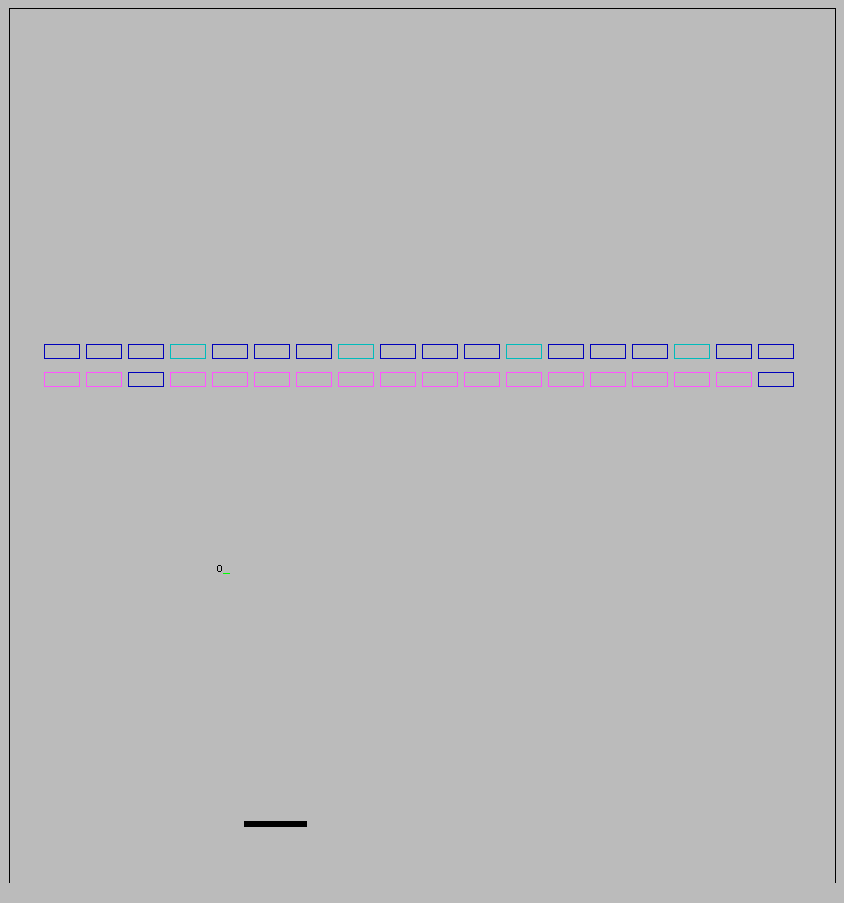
\includegraphics[scale=0.5]{img/gameplay.png}
\caption{Reflexball vist i PuTTY.}
\end{center}
\end{figure}

Programmet skal være et spil, Reflexball. Spilleren styrer en striker, som skal bruges til at reflektere en bold, således den kan bevæge sig rundt på banen. Hvis bolden rammer en af kanterne, skal bolden ligeledes også reflekteres. Hvis spilleren ikke rammer bolden ryger bolden ud af banen, og spilleren fratrækkes et liv. Såfremt spilleren ikke har flere liv tilbage, afsluttes spillet. Desuden indføres der nogle bokse i spillet, som spilleren skal ødelægge. Når spilleren har ødelagt alle disse bokse går spilleren videre til næste bane, eller vinder såfremt han er på sidste bane. Den grafiske flade bliver implementeret ved at skrive til en terminal. Ydermere får brugeren fremvist informationer fra spillet på LED'erne på boardet.





 
